\documentclass{beamer}

\mode<presentation>
{
  %\usetheme{Pittsburgh}
  \usetheme{Madrid}

  \setbeamercovered{transparent}
  % or whatever (possibly just delete it)
  \setbeamertemplate{navigation symbols}{}

  \definecolor{TLMint}{rgb}{0.00392, 0.76471, 0.65490} %01C3A7
  \usecolortheme[named=TLMint]{structure}
}


\usepackage[english]{babel}
\usepackage[utf8]{inputenc}

\usepackage{avant}
\usepackage[T1]{fontenc}
% Or whatever. Note that the encoding and the font should match. If T1
% does not look nice, try deleting the line with the fontenc.

\usepackage{mdframed}

\usepackage{algorithm2e}

\pdfinfo
{
  /CreationDate (D:20200522000755+02'00') % this is the format used by pdf for date/time
}

\title{Databases and hash tables}
\subtitle{A dive into an ancient format}
\subject{Introduction to disk-stored hash tables}
\keywords{database,hash table,dbm,disk-storage}
\author{Quentin Godfroy}
\institute{Trainline}
\date{2020-07-08}

\begin{document}

\begin{frame}
  \titlepage
\end{frame}

\section*{About the presenter}

\begin{frame}{Presentation}{About me}

  \begin{itemize}
  \item
    Connections Architect.
  \item
    Paris Office.
  \item
    I joined the company in 2012.
  \item
    As a Capitaine~Train employee.
  \item
    I work mainly on the carriers connector.
  \end{itemize}

\end{frame}

\begin{frame}{Outline}
  \tableofcontents
\end{frame}

\section{Databases}
\subsection{Generalities}

\begin{frame}{Generalities}{What do we want from databases}
\begin{block}{Thought}
Ultimately, databases store things for us. Generally on long-term storage. The choice of technology is a matter of compromise.
\end{block}

\begin{itemize}
\item speed of reads/writes/updates
\item easy queries/relational databases
\item replication
\item storage
\item data lifecycle
\end{itemize}

\begin{block}{Left-out}
Data manipulation is another very important feature of modern databases. It
is not the subject here.
\end{block}

\end{frame}

\begin{frame}{Generalities}{Some examples}
Some technology examples:
\begin{itemize}
\item MySQL, PostgreSQL, \ldots --- relational
\item Filesystems --- large storage, hierarchical, random file access
\item Object storage like S3 --- object-level access
\item NoSQLs --- key-value stores
\end{itemize}

\begin{block}{Common denominator}
Many sytems use efficient ways to locate records. One way of doing this is
the hash table.
\end{block}
\end{frame}

\subsection{Hash table}

\begin{frame}{Hash table}{Essential tool}
\begin{block}{Definition}
A hash table is one way to rapidly locate a record---the \texttt{value}---stored under a \texttt{key}.
\end{block}

\begin{block}{Basic function}
A hash function shrinks keys to a fixed size. Keys that hash together are
stored into buckets. Buckets are searched sequentially until the key is
found.
\end{block}

Virtually every storage tool uses either hash tables or b-trees.

\end{frame}

\begin{frame}{Hash table}{Hash function}
Some properties:
\begin{itemize}
\item fixed output size
\item uniformity over the result space
\item speed
\item deterministic
\item generally not injective!
\item parametrizable
\end{itemize}

\begin{block}{Warning}
Do not confuse this with a cryptographic hash. Cryptographic hashes are overkill
for this application and are generally too slow.
\end{block}
\end{frame}

\subsection{Storage}

\begin{frame}{Storage}{Memory example}

\begin{figure}
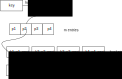
\includegraphics[scale=0.8]{hash_table.png}
\caption{Typical in memory hash table structure}
\end{figure}
\end{frame}


\begin{frame}{Storage}{Disk storage}
Why disk storage is different from memory:
\begin{itemize}
\item Orders of magnitude difference in capacity. Think kilobytes for RAM,
megabytes for disk---in the 70s. Ratio hasn't changed that much.
\item Slow random access for disks. Bad tolerance for fragmentation.
\item File API forces allocated space to be reused on disks. No
\texttt{free()}.
\end{itemize}

\begin{block}{Requirements}
We need reusable space, flat storage, low memory footprint, minimize seeks, convenient
access to data.
\end{block}
\end{frame}

\section{DBM --- DataBase Manager}
\subsection{Description}

\begin{frame}{DBM}{Description}

DBM: DataBase Manager.
\begin{itemize}
\item Introduced by Ken Thompson for Unix V7 in 1979.
\item Very early example of a NoSQL database.
\item Key-value hash table with on-disk storage.
\item Page-based. A page contains several key-value pairs.
\item Two files: \texttt{database.dir} and \texttt{database.pag}.
\item Has been used with the yellowpages directory service.
\end{itemize}

\begin{block}{Why am I talking about this?}
Interesting insight on modern databases. Old piece of technology. Curiosity.
Part of being an engineer to understand previous works.
\end{block}

\end{frame}

\begin{frame}{DBM}{Principles}
\begin{itemize}
\item Fixed page size.
\item Pages hold the key-value pairs.
\item Keys are hashed.
\item Keys with the same hash prefix are in the same page.
\item When pages overflow they are split in two.
\item The directory stores the splitting events.
\item Key lookup algorithm walks the history of splits.
\end{itemize}
\end{frame}

\begin{frame}{DBM}{Extendible hashing}
\begin{block}{Basic principle}
Keys are stored in the page \# that corresponds to its hash. Only the first
bits are considered. More bits are used as split pages are
encountered.
\end{block}

\subsection{Algorithms}

\begin{block}{Page searching}
\begin{algorithm}[H]
$hash \leftarrow hash(key)$; $mask = 0$; $page = 0$\;
\While{isSplit(hash, mask)}
{
$mask \leftarrow mask << 1 + 1$\; 
}
$page = hash\,\&\,mask$\;
\end{algorithm}
When the algorithm is finished, the key should be in the page. Or isn't and
it's not in the database.
\end{block}

\end{frame}

\begin{frame}{DBM}{Page splitting history}
Pages are split when a new key to be inserted cannot fit.
\begin{figure}
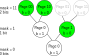
\includegraphics[scale=1]{split_pages.png}
\caption{Split history creates a binary tree. Allows to list all keys with
tree traversal.}
\end{figure}
\end{frame}

\begin{frame}{DBM}{File format}
\begin{block}{Directory}
Sea of bits. Flattened binary tree. Each level has $2^\ell$ entries. For a
mask $m$ there are exactly $m$ entries for the previous levels.
$$isSplit(hash, mask): hash \,\&\, mask + mask$$
\end{block}

\begin{block}{Pages}
\center 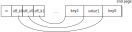
\includegraphics[scale=0.7]{dbm_page.png}
\end{block}
\end{frame}

\subsection{Limitations}

\begin{frame}{DBM}{Issues}
\begin{block}{Limitations}
\begin{itemize}
\item Keys that share the same hash have to fit in the same page.
\item Hard size limit for key + value.
\item It's a single index.
\item No concurrency
\item Two sparse files. Can appear to be pretty large.
\item Initially the library allowed only one database at a time.
\item Fixed hash function.
\end{itemize}
\end{block}

So why am I talking about this thing? Because it's one of the building
blocks of modern databases. BerkeleyDB is one of its direct descendents.
\end{frame}

\begin{frame}{Beyond DBM}
It's not very complex to imagine how we can remedy to some of the problems.

\begin{block}{Compact file}
Use more directories and indirection tables. Store the splits in a page
itself.
\end{block}

\begin{block}{Overhead pages}
Store only small data inside pages. Dedicate pages to large payloads.
\end{block}

\begin{block}{Hashing}
Use parametrizable hashing.
\end{block}

\end{frame}

\begin{frame}{End}
\begin{itemize}
\item Thank you.
\item Don't forget to give feedbacks. \texttt{!summit} on slack.
\end{itemize}
\end{frame}

\end{document}
